% !TEX root = ../Tesis_NataliaOpazo.tex 


\begin{figure}[H]
\centering
 \includegraphics[width=1.2\textwidth]{../../Figuras/Spin-up/Ingles/SPIN-UP}
 \caption[Simulación spin-up]{Serie de pCO$_2$ obtenidos a partir de las simulaciones spin-up realizadas mediante el modelo cGENIE, para el periodo que va desde el Holoceno hasta el UMG. La primera fila muestra la temperatura superficial, mientra la segunda fila presenta la temperatura de fondo para todos los casos.}
  \label{fig:SPIN-UP}
\end{figure}
\newpage

 \begin{figure}[H]
        \begin{subfigure}[b]{0.55\textwidth}
                \includegraphics[width=\linewidth]{../../Figuras/Amplitud/Albani_amplitud2.pdf}
                \caption{Lambert}
                \label{fig:L}
        \end{subfigure}%
        \begin{subfigure}[b]{0.55\textwidth}
                \includegraphics[width=\linewidth]{../../Figuras/Amplitud/Lambert_Amplitud2.pdf}
                \caption{Albani}
                \label{fig:A}
        \end{subfigure}%
        
        \begin{subfigure}[b]{0.55\textwidth}
                \includegraphics[width=\linewidth]{../../Figuras/Amplitud/MIROC_Amplitud2.pdf}
                \caption{Takemura}
                \label{fig:T}
        \end{subfigure}%
        \begin{subfigure}[b]{0.55\textwidth}
                \includegraphics[width=\linewidth]{../../Figuras/Amplitud/MRI-CGCM3_Amplitud2.pdf}
                \caption{MIROC-ESM}
                \label{fig:MI}
        \end{subfigure}
        
        \begin{subfigure}[b]{0.55\textwidth}
                \includegraphics[width=\linewidth]{../../Figuras/Amplitud/Takemura_Amplitud2.pdf}
                \caption{MRI-CGCM3}
                \label{fig:MR}
        \end{subfigure}
        \caption[Amplitud flujos de polvo]{Diferencia de flujos de polvo entre el UMG y el Holoceno}\label{fig:Amp}
\end{figure}

\newpage

Este proceso es llevado a cabo con el fin de posterior a las corridas cGENIE, graficar los datos de CO$_2$ obtenidos con respecto a la masa de polvo que se deposita en una celda de las regiones HNLC cada año. Así, posteriormente sumamos los valores para una regi\'on y tenemos la masa total de polvo que se deposita por año en esta zona. 

Para obtener una fracci\'on de \'area de la tierra en funci\'on de una latitud y longitud determinada, vamos a considerar la tierra una esfera de tipo
  elipsoide (figura \ref{fig:mundo1_met}). Donde la ecuaci\'on \ref{eq:met2} nos permiti\'o obtener dicha \'area. 
  \begin{equation} \label{eq:met2}
   A_{sup}=\displaystyle\int_{\varphi_1}^{\varphi_2} R \left( \displaystyle\int_{\lambda_2}^{\lambda_2} R\ cos\varphi\ d\lambda \right) d\varphi = R^{2} 
  \left(\lambda_2 - \lambda_1 \right) \left(sen\varphi_2 - sen\varphi_1 \right) 
  \end{equation}
  
   Donde R es el radio de la tierra (apr\'oximadamente 6371 km); y donde\\
   $ 0\leqq \lambda_1 \leqq \lambda \leqq \lambda_2 \leqq 2\pi $ y donde, $ \frac{-\pi}{2} \leqq \varphi_1 \leqq \varphi \leqq \varphi_2 \leqq \frac{\pi}{2}$.
  
  \begin{figure}[H]
  \centering
  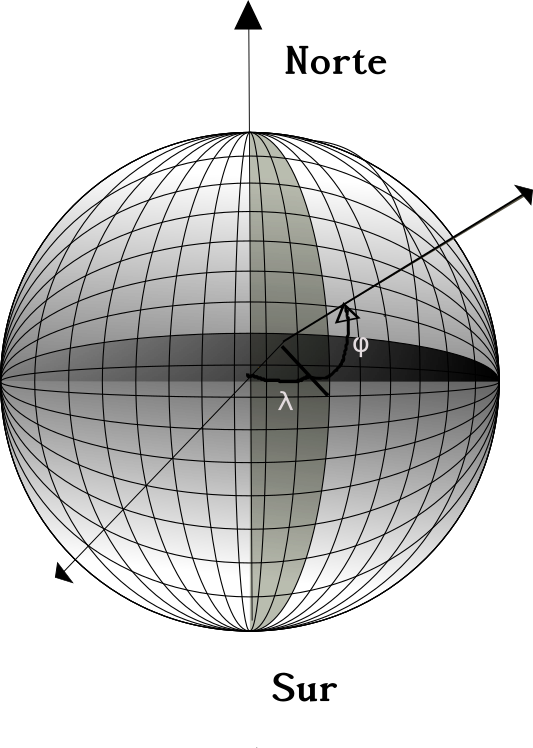
\includegraphics[width=0.3\textwidth]{mundo1_met.png}
  \caption[Área superficial de una grilla]{\'Area superficial de una celda de grilla entre longitudes $ \lambda_1\ y\ \lambda_2 $ y latitudes $ \varphi_1\ y\ \varphi_2$.}
  \label{fig:mundo1_met}
\end{figure}

 Para realizar el calculo anterior se ocupo una funci\'on MATLAB denomina \textit{areaquad} y los datos de longitud y latitud de cuadrantes especificados en
 la tabla \ref{tabla:Area1}. As\'i los resultados son expresado en unidades de metros cuadrados ($m^{2}$).

 \newpage

\begin{table}[H] 
\centering
\resizebox{16cm}{!} {%
\begin{tabular}{|ccc|}
\hline \hline
\multicolumn{3}{c}{\bf Configuración cGENIE} \\
%\cline{2}
\hline \hline
{\bf Componentes} & {\bf Prescripción} & {\bf Dato} \\
\hline \hline
CLIMA  & Retroalimentación  & Si\\ \hline
\multirow{4}{*}{\makecell{ESQUEMA DE PRODUCCIÓN \\ BIOLÓGICA NUEVA}} &
\makecell{Identificador de esquema \\ de exportación} & \makecell{$bio\_PFe$ (Plancton \\ no silíceo)} \\ \cline{2-3}
& Valor de saturación media PO4 & 0.10e$-6$ [mol kg$^{-1}$]\\ \cline{2-3}
& Valor de saturación media de Fe & 0.10E-09 [mol kg$^{-1}$]\\ \cline{2-3}
& \makecell{Escala de tiempo de absorción \\ de nutrientes  (por el plancton)} & 63.3827 \\ \hline
\makecell{TASA DE MATERIA ORGÁNICA \\ EXPORTADA} & \makecell{Fracción de producción de \\ materia orgánica disuelta} & 0.66 \\ \hline
\multirow{2}{*}{\makecell{TASA DE MATERIA INORGÁNICA\\ EXPORTADA}} & \makecell{Relación de exportación \\biológica CaCO3/POC}  & 0.0485 \\ \cline{2-3}
& {Estado de saturación ambiental} & 0.7440\\ \hline
\multirow{7}{*}{REMINERALIZACIÓN} & Tiempo de vida del DOC [años] & 1 \\ \cline{2-3}
& \makecell{Fraccionamiento de la \\ abundancia inicial del DOC} & 0.055 \\ \cline{2-3}
& \makecell{Profundidad de la remineralización\\ o POC}& 589.9451 \\ \cline{2-3}
& Longitud de la remineralización del POC & 1000000 \\ \cline{2-3}
& \makecell{Fraccionamiento de la \\ abundancia inicial del CACO3} & 0.45 \\ \cline{2-3}
& \makecell{Profundidad de la remineralización\\ o CACO3} & 1.8905e+3\\ \cline{2-3}
& Longitud de la remineralización del CaCO3 & 1000000\\ \hline
\multirow{11}{*}{HIERRO} & Solubilidad eólica & 0.00291468 \\ \cline{2-3}
& \makecell{Exponente de la solubilidad\\ del hierro} & \makecell{0.5 (1 en caso \\ de ser uniforme)}\\ \cline{2-3}
& \makecell{Modificador de la tasa de \\ eliminación de hierro disuelto} & \makecell{para el POC=1.338130\\
para el CaCO3=0; para el opalo=0\\
para el hierro=0}  \\ \cline{2-3} 
& Regeneración sin barrido & 0 \\ \cline{2-3}
& Retorno de POFe & No \\ \cline{2-3}
& Fe:C Variable & NO \\ \cline{2-3}
& Ajustar pk'(Fel) & 11 \\ \cline{2-3}
& \makecell{Máxima tasa de \\ materia orgánica} & 250000 \\ \cline{2-3}
& Tasa de dependencia Fe:C & \makecell{FetoC pP=-0.4225; \\
 FetoC K=103684; Fetoc C=0} \\ \hline
\multirow{2}{*}{FORZANTES} & Especificación de Forzante & Archivo base\_config \\ \cline{2-3}
& Concentración atmosférica de CO$_2$ & \makecell{278$e^{-6}$ (spin-up) o no \\ definido (simulaciones considerando el polvo)}  \\ \hline \hline 
\end{tabular}%
}
\caption[Configuración cGENIE]{Configuración ``User\_config'' del modelo cGENIE. } 
\label{tabla:U-conf}
\end{table} 
